\documentclass[12pt,a4paper]{article}

% -------------------------------------------------------
%  Packages
% -------------------------------------------------------
\usepackage{amsmath}
\usepackage{amssymb}
\usepackage{geometry}
\geometry{margin=2.5cm}
\usepackage{booktabs}
\usepackage{xcolor}
\usepackage{hyperref}
\usepackage{listings}
\usepackage{pgfplots}
\pgfplotsset{compat=1.18}
\usepackage[skins,breakable]{tcolorbox}
\usepackage{enumitem}
\usepackage{fancyhdr}
\usepackage{tikz}
\usepackage{array}

% -------------------------------------------------------
%  tcolorbox environments
% -------------------------------------------------------
\newtcolorbox{curiositybox}[1]{colback=yellow!10, colframe=orange!80!black, fonttitle=\bfseries, title=#1, breakable}
\newtcolorbox{infobox}[1]{colback=blue!5, colframe=blue!60!black, fonttitle=\bfseries, title=#1, breakable}
\newtcolorbox{mistakebox}[1]{colback=red!5, colframe=red!60!black, fonttitle=\bfseries, title=#1, breakable}
\newtcolorbox{learnbox}[1]{colback=green!5, colframe=green!60!black, fonttitle=\bfseries, title=#1, breakable}

% -------------------------------------------------------
%  lstlisting (Python)
% -------------------------------------------------------
\lstset{language=Python, basicstyle=\ttfamily\small, keywordstyle=\color{blue},
        commentstyle=\color{gray}, stringstyle=\color{red},
        showstringspaces=false, breaklines=true, frame=single}

% -------------------------------------------------------
%  fancyhdr
% -------------------------------------------------------
\pagestyle{fancy}
\fancyhf{}
\lhead{Topic 16: Laurent Series}
\rhead{Unit II --- Complex Variables}
\cfoot{\thepage}

% -------------------------------------------------------
%  Title
% -------------------------------------------------------
\title{\textbf{Topic 16: Laurent's Series}\\[6pt]
       \large Unit II --- Complex Variable: Integration\\
       Complex Variables and Special Functions\\
       JNTUA College of Engineering (Autonomous)}
\author{B.Tech Engineering --- Lecture Notes}
\date{}

% -------------------------------------------------------
\begin{document}
% -------------------------------------------------------
\maketitle
\tableofcontents
\newpage

% ====================================================
%  Opening Hook
% ====================================================
\begin{curiositybox}{Hook}
Taylor series are perfect when a function is analytic at the center. But what if the
function has a singularity there? Laurent series rescue the situation by allowing negative
powers, and those negative powers reveal the exact nature of the singularity.
\end{curiositybox}

\bigskip

% ====================================================
\section{Why Taylor Series Is Not Enough}
% ====================================================

\subsection*{Motivation}

A Taylor series represents a function $f(z)$ as a power series in non-negative powers of
$(z - z_0)$. This requires $f$ to be analytic at and near $z_0$. Consider $f(z)=\dfrac{1}{z}$.

\begin{itemize}
  \item $f(z)$ is analytic everywhere \textbf{except} at $z=0$.
  \item No Taylor series centred at $z_0 = 0$ exists because $f$ is not analytic there.
  \item However, the function is perfectly well-behaved on any annulus
        $0 < |z| < R$ for any $R > 0$.
\end{itemize}

\begin{center}
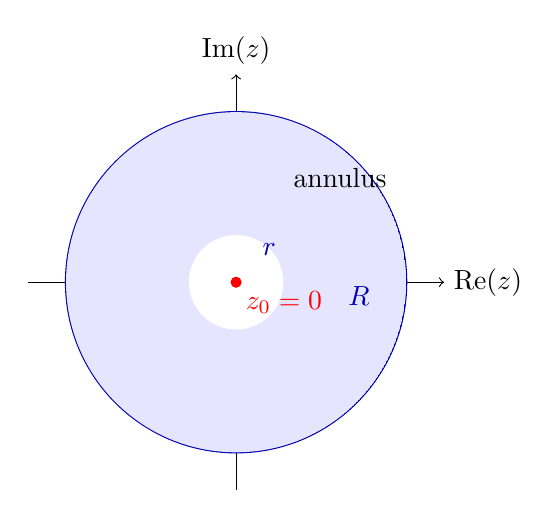
\begin{tikzpicture}[scale=1.2]
  % Axes
  \draw[->] (-2.2,0) -- (2.2,0) node[right] {$\operatorname{Re}(z)$};
  \draw[->] (0,-2.2) -- (0,2.2) node[above] {$\operatorname{Im}(z)$};
  % Inner circle (singularity excluded)
  \draw[dashed, blue!70!black, thick] (0,0) circle (0.5);
  % Outer circle (boundary of annulus)
  \draw[blue!70!black, thick] (0,0) circle (1.8);
  % Shading annular region
  \begin{scope}
    \clip (0,0) circle (1.8);
    \fill[blue!10] (0,0) circle (1.8);
    \fill[white]   (0,0) circle (0.5);
  \end{scope}
  % Singularity
  \filldraw[red] (0,0) circle (1.5pt) node[below right] {$z_0=0$};
  % Labels
  \node at (1.1,1.1) {annulus};
  \node[blue!70!black] at (0.35,0.35) {$r$};
  \node[blue!70!black] at (1.3,-0.15) {$R$};
\end{tikzpicture}
\end{center}

\noindent
Trying $f(z)=1/z$ as a Taylor series at $z=0$: the coefficient formula
$a_n = f^{(n)}(0)/n!$ is undefined because $f$ is not analytic at $0$.
We need a more general expansion that admits \emph{negative} powers of $z$.

\begin{center}
\begin{tabular}{lll}
\toprule
\textbf{Aspect} & \textbf{Taylor Series} & \textbf{Laurent Series} \\
\midrule
Center $z_0$ & Must be analytic & May have singularity \\
Powers used & $0, 1, 2, \ldots$ & $\ldots, -2, -1, 0, 1, 2, \ldots$ \\
Convergence region & Disk $|z-z_0|<R$ & Annulus $r<|z-z_0|<R$ \\
Existence condition & $f$ analytic at $z_0$ & $f$ analytic on the annulus \\
\bottomrule
\end{tabular}
\end{center}

\begin{learnbox}{Key Takeaway}
Taylor series fail at singularities. Laurent series extend the idea to annular regions by
including negative powers of $(z-z_0)$, making them indispensable near singular points.
\end{learnbox}

% ====================================================
\section{Statement / Form of Laurent Series}
% ====================================================

\begin{infobox}{Laurent's Theorem}
Let $f(z)$ be analytic on the annular region
$r < |z - z_0| < R$ (where $0 \leq r < R \leq \infty$).
Then $f(z)$ can be represented uniquely as:
\[
  f(z) = \sum_{n=-\infty}^{\infty} a_n (z-z_0)^n
       = \cdots + \frac{a_{-2}}{(z-z_0)^2} + \frac{a_{-1}}{z-z_0}
         + a_0 + a_1(z-z_0) + a_2(z-z_0)^2 + \cdots
\]
where the coefficients are given by:
\[
  a_n = \frac{1}{2\pi i} \oint_{C} \frac{f(z)}{(z-z_0)^{n+1}}\,dz,
  \qquad n = 0, \pm 1, \pm 2, \ldots
\]
and $C$ is any simple closed contour lying in the annulus, traversed counterclockwise.
\end{infobox}

\subsection*{Annular Region of Convergence}

The series converges absolutely and uniformly on any closed sub-annulus
$r < r_1 \leq |z-z_0| \leq R_1 < R$.
The inner radius $r$ is determined by the nearest singularity \emph{inside} or at $z_0$,
and the outer radius $R$ by the nearest singularity \emph{outside} the annulus.

\begin{learnbox}{Annulus Intuition}
Think of peeling away the singularity: the inner circle of the annulus surrounds the singular
point, while the outer circle is kept inside the next singularity. Laurent series live in
exactly this gap.
\end{learnbox}

% ====================================================
\section{Principal Part and Analytic Part}
% ====================================================

\begin{infobox}{Decomposition of Laurent Series}
Given $\displaystyle f(z) = \sum_{n=-\infty}^{\infty} a_n(z-z_0)^n$, we split it into:

\textbf{Principal Part:}
\[
  P(z) = \sum_{n=1}^{\infty} \frac{a_{-n}}{(z-z_0)^n}
       = \frac{a_{-1}}{z-z_0} + \frac{a_{-2}}{(z-z_0)^2} + \cdots
\]
Contains all \emph{negative} powers of $(z-z_0)$. Encodes the singular behaviour.

\textbf{Analytic Part (Regular Part):}
\[
  A(z) = \sum_{n=0}^{\infty} a_n(z-z_0)^n
       = a_0 + a_1(z-z_0) + a_2(z-z_0)^2 + \cdots
\]
Contains all \emph{non-negative} powers; this is a Taylor-like series analytic at $z_0$.

So $f(z) = P(z) + A(z)$ on the annulus.
\end{infobox}

\noindent\textbf{Example.} For $f(z)=\dfrac{e^z}{z^3}$ near $z=0$:
\[
  f(z) = \frac{1}{z^3}\left(1 + z + \frac{z^2}{2!} + \frac{z^3}{3!} + \cdots\right)
       = \underbrace{\frac{1}{z^3} + \frac{1}{z^2} + \frac{1}{2z}}_{\text{principal part}}
         + \underbrace{\frac{1}{6} + \frac{z}{24} + \cdots}_{\text{analytic part}}.
\]

\begin{learnbox}{Principal vs.\ Analytic Part}
The principal part is the ``singular fingerprint'' of $f$ at $z_0$. The analytic part
converges near $z_0$ and contains no singular information.
\end{learnbox}

% ====================================================
\section{Connection with Singularity Classification}
% ====================================================

\begin{infobox}{Singularities via Laurent Series}
The structure of the principal part at an isolated singularity $z_0$ classifies it:

\medskip
\begin{tabular}{lll}
\toprule
\textbf{Singularity Type} & \textbf{Principal Part} & \textbf{Example} \\
\midrule
Removable singularity & All $a_{-n}=0$ (no negative powers) & $\dfrac{\sin z}{z}$ at $z=0$ \\[6pt]
Pole of order $m$ & Finitely many: $a_{-m}\neq 0$, $a_{-n}=0$ for $n>m$ & $\dfrac{1}{(z-1)^3}$ at $z=1$ \\[6pt]
Simple pole & $m=1$: only $a_{-1}\neq 0$ in principal part & $\dfrac{1}{z-2}$ at $z=2$ \\[6pt]
Essential singularity & Infinitely many non-zero $a_{-n}$ & $e^{1/z}$ at $z=0$ \\
\bottomrule
\end{tabular}
\end{infobox}

\noindent\textbf{Key remark.} The residue of $f$ at $z_0$ is exactly $a_{-1}$, the
coefficient of $(z-z_0)^{-1}$ in the Laurent expansion --- this is why Laurent series are
central to residue calculations.

\begin{learnbox}{Singularity Classification Summary}
Count the number of negative-power terms in the Laurent series: zero $\Rightarrow$ removable,
finite $\Rightarrow$ pole (order = highest negative index), infinite $\Rightarrow$ essential.
\end{learnbox}

% ====================================================
\section{Methods of Expansion}
% ====================================================

There are four standard techniques for obtaining Laurent series without evaluating the
contour-integral formula directly.

\subsection*{Method 1: Algebraic Rewriting}

Write $f(z)$ so that the singular factor is isolated, then expand the remaining part as a
Taylor series.

\textbf{Example.} $f(z) = \dfrac{\cos z}{z^2}$ about $z=0$.

\[
  \cos z = 1 - \frac{z^2}{2!} + \frac{z^4}{4!} - \cdots
  \implies
  \frac{\cos z}{z^2} = \frac{1}{z^2} - \frac{1}{2} + \frac{z^2}{24} - \cdots
\]

\subsection*{Method 2: Geometric-Series Expansion}

Use $\dfrac{1}{1-w} = \sum_{n=0}^{\infty} w^n$ for $|w|<1$
and $\dfrac{1}{1-w} = -\dfrac{1}{w}\dfrac{1}{1-1/w}
= -\sum_{n=0}^{\infty} w^{-(n+1)}$ for $|w|>1$.

\textbf{Example.} $f(z)=\dfrac{1}{z-2}$ about $z=0$.

\begin{itemize}
  \item Region $|z|<2$: $\dfrac{1}{z-2} = -\dfrac{1}{2}\cdot\dfrac{1}{1-z/2}
        = -\dfrac{1}{2}\sum_{n=0}^{\infty}\left(\dfrac{z}{2}\right)^n$
        (Taylor series --- no principal part).
  \item Region $|z|>2$: $\dfrac{1}{z-2} = \dfrac{1}{z}\cdot\dfrac{1}{1-2/z}
        = \dfrac{1}{z}\sum_{n=0}^{\infty}\left(\dfrac{2}{z}\right)^n
        = \sum_{n=0}^{\infty}\dfrac{2^n}{z^{n+1}}$ (Laurent series).
\end{itemize}

\subsection*{Method 3: Partial Fractions}

Decompose $f(z)$ into simpler fractions, then expand each piece in the required region.

\textbf{Example.} $f(z)=\dfrac{1}{(z-1)(z-3)}$. Partial fractions:
$\dfrac{1}{2}\left(\dfrac{1}{z-3}-\dfrac{1}{z-1}\right)^{-1}$
--- each term is expanded separately depending on which region is specified.

\subsection*{Method 4: Region-Driven Expansion}

The \emph{same} function can have \emph{different} Laurent series in different annuli. The
region $r < |z-z_0| < R$ determines which geometric-series formula applies to each factor.

\begin{learnbox}{Choosing the Right Method}
Always identify the region first. Then decide which factor to expand: if a factor $1/(z-a)$
has $|z-a|<1$ in your region use positive-power geometric series; if $|z-a|>1$ use
negative-power series. Partial fractions help when multiple poles are present.
\end{learnbox}

% ====================================================
\section{Worked Examples}
% ====================================================

% ------ Example 1 ------
\subsection*{Example 1: $f(z)=\dfrac{1}{z}$, centre $z_0=0$}

Region: $0 < |z| < \infty$.

\[
  f(z) = \frac{1}{z}.
\]
This is already in Laurent form: $a_{-1}=1$, all other $a_n=0$.\\
Principal part: $\dfrac{1}{z}$. Simple pole at $z=0$. Residue $= 1$.

\begin{learnbox}{Example 1 Result}
$1/z$ is its own Laurent series; the single negative-power term confirms a simple pole at $z=0$.
\end{learnbox}

% ------ Example 2 ------
\subsection*{Example 2: $f(z)=\dfrac{e^z}{z^2}$, centre $z_0=0$}

Region: $0 < |z| < \infty$.

Use $e^z = \sum_{n=0}^{\infty} \dfrac{z^n}{n!}$:
\[
  \frac{e^z}{z^2} = \frac{1}{z^2}\left(1 + z + \frac{z^2}{2}+\frac{z^3}{6}+\cdots\right)
  = \frac{1}{z^2} + \frac{1}{z} + \frac{1}{2} + \frac{z}{6} + \frac{z^2}{24} + \cdots
\]
Principal part: $\dfrac{1}{z^2}+\dfrac{1}{z}$. This is a pole of order 2 at $z=0$.
Residue $= a_{-1} = 1$.

\begin{learnbox}{Example 2 Result}
Dividing a convergent power series by $z^n$ shifts all indices down by $n$, producing an order-$n$ pole; the residue is the coefficient of $z^{-1}$.
\end{learnbox}

% ------ Example 3 ------
\subsection*{Example 3: $f(z)=\dfrac{\sin z}{z^3}$, centre $z_0=0$}

Region: $0 < |z| < \infty$.

\[
  \sin z = z - \frac{z^3}{6} + \frac{z^5}{120} - \cdots
\]
\[
  \frac{\sin z}{z^3} = \frac{1}{z^2} - \frac{1}{6} + \frac{z^2}{120} - \cdots
\]
Principal part: $\dfrac{1}{z^2}$ only. Pole of order 2. Residue $= 0$ (coefficient of $z^{-1}$ is $0$).

\begin{learnbox}{Example 3 Result}
Even with a high-order denominator, the residue can be zero; always read off $a_{-1}$ explicitly.
\end{learnbox}

% ------ Example 4 ------
\subsection*{Example 4: $f(z)=e^{1/z}$, centre $z_0=0$}

Region: $0 < |z| < \infty$.

Let $w=1/z$. Then $e^w = \sum_{n=0}^{\infty} \dfrac{w^n}{n!}$, so:
\[
  e^{1/z} = 1 + \frac{1}{z} + \frac{1}{2!\,z^2} + \frac{1}{3!\,z^3} + \cdots
\]
The principal part has \emph{infinitely many} non-zero terms: $\dfrac{1}{z}, \dfrac{1}{2z^2}, \ldots$
This is an \textbf{essential singularity} at $z=0$. Residue $= a_{-1} = 1$.

\begin{learnbox}{Example 4 Result}
$e^{1/z}$ is the textbook essential singularity. Its Laurent series never terminates; this is the defining property of essential singularities.
\end{learnbox}

% ------ Example 5 ------
\subsection*{Example 5: $f(z)=\dfrac{1}{z(z-1)}$ in region $0<|z|<1$}

Partial fractions: $\dfrac{1}{z(z-1)} = \dfrac{-1}{z} + \dfrac{1}{z-1}$.

In region $0 < |z| < 1$ we have $|z|<1$, so expand $\dfrac{1}{z-1} = -\dfrac{1}{1-z}$:
\[
  \frac{1}{z-1} = -\frac{1}{1-z} = -\sum_{n=0}^{\infty} z^n \quad (|z|<1).
\]
Therefore:
\[
  f(z) = -\frac{1}{z} - \sum_{n=0}^{\infty} z^n
       = -\frac{1}{z} - 1 - z - z^2 - z^3 - \cdots
\]
Principal part: $-\dfrac{1}{z}$. Simple pole. Residue $= -1$.

\begin{learnbox}{Example 5 Result}
In the punctured disk $0<|z|<1$, the singularity at $z=0$ dominates and gives a simple pole with residue $-1$.
\end{learnbox}

% ------ Example 6 ------
\subsection*{Example 6: $f(z)=\dfrac{1}{z(z-1)}$ in region $|z|>1$}

Using partial fractions from Example 5: $f(z) = \dfrac{-1}{z}+\dfrac{1}{z-1}$.

In region $|z|>1$, expand $\dfrac{1}{z-1} = \dfrac{1}{z}\cdot\dfrac{1}{1-1/z}$:
\[
  \frac{1}{z-1} = \frac{1}{z}\sum_{n=0}^{\infty}\frac{1}{z^n} = \sum_{n=0}^{\infty}\frac{1}{z^{n+1}} \quad (|z|>1).
\]
Therefore:
\[
  f(z) = -\frac{1}{z} + \sum_{n=0}^{\infty}\frac{1}{z^{n+1}}
       = -\frac{1}{z} + \frac{1}{z} + \frac{1}{z^2} + \frac{1}{z^3} + \cdots
       = \sum_{n=2}^{\infty}\frac{1}{z^n}
       = \frac{1}{z^2} + \frac{1}{z^3} + \cdots
\]
No simple pole term ($a_{-1}=0$). Residue at $z=0$ from this expansion $= 0$.

\begin{learnbox}{Example 6 Result}
The \emph{same} function $1/[z(z-1)]$ has a completely different Laurent expansion in $|z|>1$. The residue as seen from this outer region is $0$ because $z=0$ is inside the contour, not on the annulus boundary.
\end{learnbox}

% ------ Example 7 ------
\subsection*{Example 7: $f(z)=\dfrac{1}{(z-1)(z-3)}$ in $1<|z|<3$}

Partial fractions: $\dfrac{1}{(z-1)(z-3)} = \dfrac{-1/2}{z-1} + \dfrac{1/2}{z-3}$.

Region $1 < |z| < 3$ means $|z|>1$ (expand $(z-1)^{-1}$ in negative powers of $z$)
and $|z|<3$ (expand $(z-3)^{-1}$ in positive powers of $z/3$).

\[
  \frac{1}{z-1} = \frac{1}{z}\cdot\frac{1}{1-1/z} = \frac{1}{z}\sum_{n=0}^{\infty}\frac{1}{z^n}
               = \sum_{n=0}^{\infty}\frac{1}{z^{n+1}} \quad (|z|>1),
\]
\[
  \frac{1}{z-3} = -\frac{1}{3}\cdot\frac{1}{1-z/3} = -\frac{1}{3}\sum_{n=0}^{\infty}\frac{z^n}{3^n}
               = -\sum_{n=0}^{\infty}\frac{z^n}{3^{n+1}} \quad (|z|<3).
\]
Therefore:
\[
  f(z) = -\frac{1}{2}\sum_{n=0}^{\infty}\frac{1}{z^{n+1}}
         -\frac{1}{2}\sum_{n=0}^{\infty}\frac{z^n}{3^{n+1}}.
\]
Residue at $z=1$ (from $a_{-1}$ of first sum, $n=0$): $a_{-1} = -\dfrac{1}{2}$.

\begin{learnbox}{Example 7 Result}
When two poles bracket the annulus, one factor is expanded in positive powers and the other in negative powers, determined strictly by which side of the annulus boundary each pole lies on.
\end{learnbox}

% ------ Example 8 ------
\subsection*{Example 8: $f(z)=\dfrac{z+1}{z^2-3z+2}$ about $z_0=0$, region $1<|z|<2$}

Factor denominator: $z^2-3z+2 = (z-1)(z-2)$.

Partial fractions: $\dfrac{z+1}{(z-1)(z-2)}$. Let
$\dfrac{z+1}{(z-1)(z-2)} = \dfrac{A}{z-1}+\dfrac{B}{z-2}$.

$A(z-2)+B(z-1)=z+1$.\\
At $z=1$: $A(-1) = 2 \Rightarrow A = -2$.\\
At $z=2$: $B(1) = 3 \Rightarrow B = 3$.

So $f(z) = \dfrac{-2}{z-1} + \dfrac{3}{z-2}$.

Region $1 < |z| < 2$: expand $\dfrac{1}{z-1}$ for $|z|>1$ and $\dfrac{1}{z-2}$ for $|z|<2$.

\[
  \frac{1}{z-1} = \frac{1}{z}\sum_{n=0}^{\infty}\frac{1}{z^n} = \sum_{n=0}^{\infty}\frac{1}{z^{n+1}},
\]
\[
  \frac{1}{z-2} = -\frac{1}{2}\cdot\frac{1}{1-z/2} = -\frac{1}{2}\sum_{n=0}^{\infty}\frac{z^n}{2^n}
               = -\sum_{n=0}^{\infty}\frac{z^n}{2^{n+1}}.
\]
Therefore:
\[
  f(z) = -2\sum_{n=0}^{\infty}\frac{1}{z^{n+1}} + 3\left(-\sum_{n=0}^{\infty}\frac{z^n}{2^{n+1}}\right)
       = -2\sum_{n=0}^{\infty}\frac{1}{z^{n+1}} - \frac{3}{2}\sum_{n=0}^{\infty}\frac{z^n}{2^{n}}.
\]
Residue $= a_{-1}$: coefficient of $z^{-1}$ from $-2\sum \frac{1}{z^{n+1}}$ at $n=0$ is $-2$.
Residue $= -2$.

\begin{learnbox}{Example 8 Result}
After partial fractions, expanding each piece in the given annulus yields the full Laurent series; the residue $a_{-1}$ is read from the $z^{-1}$ term of the negative-power sum.
\end{learnbox}

% ====================================================
\section{Region-Sensitive Expansion Table (MANDATORY UPGRADE)}
% ====================================================

The following table catalogues how representative functions expand differently depending on
the annular region chosen.

\begin{center}
\begin{tabular}{p{3.2cm} p{1.5cm} p{3.5cm} p{5cm}}
\toprule
\textbf{Function} & \textbf{Centre} & \textbf{Region} & \textbf{Resulting Series Form} \\
\midrule
$\dfrac{1}{z(z-1)}$
  & $z_0=0$
  & $0<|z|<1$
  & $\displaystyle -\frac{1}{z}-\sum_{n=0}^{\infty}z^n$ (simple pole, principal part $-1/z$) \\[14pt]

$\dfrac{1}{z(z-1)}$
  & $z_0=0$
  & $|z|>1$
  & $\displaystyle \sum_{n=2}^{\infty}\frac{1}{z^n}$ (all negative powers, no simple pole term) \\[14pt]

$\dfrac{1}{(z-1)(z-3)}$
  & $z_0=0$
  & $1<|z|<3$
  & Mixed: neg.\ powers from $(z-1)^{-1}$; pos.\ powers from $(z-3)^{-1}$ \\[14pt]

$\dfrac{1}{(z-1)(z-3)}$
  & $z_0=0$
  & $|z|>3$
  & $\displaystyle \sum_{n=0}^{\infty}\frac{c_n}{z^{n+2}}$ (all negative powers $\geq z^{-2}$) \\[14pt]

$\dfrac{1}{z-a}$, $a\neq 0$
  & $z_0=0$
  & $|z|<|a|$
  & $\displaystyle -\frac{1}{a}\sum_{n=0}^{\infty}\left(\frac{z}{a}\right)^n$ (Taylor, no principal part) \\[14pt]

$\dfrac{1}{z-a}$, $a\neq 0$
  & $z_0=0$
  & $|z|>|a|$
  & $\displaystyle \frac{1}{z}\sum_{n=0}^{\infty}\left(\frac{a}{z}\right)^n$ (Laurent, principal part $\sim 1/z$) \\[14pt]

$e^{1/z}$
  & $z_0=0$
  & $0<|z|<\infty$
  & $\displaystyle 1+\frac{1}{z}+\frac{1}{2!z^2}+\cdots$ (essential singularity, infinite principal part) \\[14pt]

$\dfrac{\sin z}{z^4}$
  & $z_0=0$
  & $0<|z|<\infty$
  & $\displaystyle \frac{1}{z^3}-\frac{1}{6z}+\frac{z}{120}-\cdots$ (pole of order 3, residue $= -1/6$) \\[14pt]

$\dfrac{z+1}{(z-1)(z-2)}$
  & $z_0=0$
  & $1<|z|<2$
  & $\displaystyle -2\sum\frac{1}{z^{n+1}} - \frac{3}{2}\sum\frac{z^n}{2^n}$ (as in Example 8) \\
\bottomrule
\end{tabular}
\end{center}

\begin{learnbox}{Region-Sensitive Insight}
The Laurent expansion of a rational function is \emph{not unique}; specifying the region is as
important as specifying the function and centre. Always state the region before writing any
expansion.
\end{learnbox}

% ====================================================
\section{Excel Example (MANDATORY)}
% ====================================================

\subsection*{Partial Sums of Laurent Series in an Annulus}

We approximate $f(z) = \dfrac{1}{z(z-1)}$ along the circle $|z| = 0.5$ (inside the annulus
$0 < |z| < 1$) using the expansion $f(z) = -\dfrac{1}{z} - 1 - z - z^2 - \cdots$

Truncate at the $N$-th partial sum:
\[
  S_N(z) = -\frac{1}{z} - \sum_{n=0}^{N} z^n.
\]
We use real $z = x > 0$ for numerical illustration.

\subsubsection*{Spreadsheet Setup}

\begin{center}
\begin{tabular}{ccccccc}
\toprule
\textbf{Col A} & \textbf{Col B} & \textbf{Col C} & \textbf{Col D} & \textbf{Col E} & \textbf{Col F} & \textbf{Col G}\\
$x$ & $f(x)$ exact & $S_2(x)$ & $S_4(x)$ & $S_6(x)$ & $S_8(x)$ & Error $|f - S_8|$ \\
\midrule
0.1 & \texttt{=1/(A2*(A2-1))} & \texttt{=-1/A2-1-A2-A2\^{}2} & \texttt{=C2-A2\^{}3-A2\^{}4} & \texttt{=D2-A2\^{}5-A2\^{}6} & \texttt{=E2-A2\^{}7-A2\^{}8} & \texttt{=ABS(B2-F2)} \\
0.2 & \texttt{=1/(A3*(A3-1))} & \texttt{=-1/A3-1-A3-A3\^{}2} & \texttt{=C3-A3\^{}3-A3\^{}4} & \texttt{=D3-A3\^{}5-A3\^{}6} & \texttt{=E3-A3\^{}7-A3\^{}8} & \texttt{=ABS(B3-F3)} \\
0.3 & \texttt{=1/(A4*(A4-1))} & \texttt{=-1/A4-1-A4-A4\^{}2} & \texttt{=C4-A4\^{}3-A4\^{}4} & \texttt{=D4-A4\^{}5-A4\^{}6} & \texttt{=E4-A4\^{}7-A4\^{}8} & \texttt{=ABS(B4-F4)} \\
0.4 & \texttt{=1/(A5*(A5-1))} & \texttt{=-1/A5-1-A5-A5\^{}2} & \texttt{=C5-A5\^{}3-A5\^{}4} & \texttt{=D5-A5\^{}5-A5\^{}6} & \texttt{=E5-A5\^{}7-A5\^{}8} & \texttt{=ABS(B5-F5)} \\
\bottomrule
\end{tabular}
\end{center}

\subsubsection*{Sample Computed Values}

\begin{center}
\begin{tabular}{ccccccc}
\toprule
$x$ & $f(x)$ & $S_2$ & $S_4$ & $S_6$ & $S_8$ & Error \\
\midrule
0.1 & $-11.111$ & $-11.210$ & $-11.111$ & $-11.111$ & $-11.111$ & $< 0.001$ \\
0.2 & $-6.250$  & $-6.440$  & $-6.256$  & $-6.250$  & $-6.250$  & $< 0.001$ \\
0.3 & $-4.762$  & $-5.043$  & $-4.771$  & $-4.762$  & $-4.762$  & $< 0.001$ \\
0.4 & $-4.167$  & $-4.566$  & $-4.182$  & $-4.167$  & $-4.167$  & $< 0.001$ \\
\bottomrule
\end{tabular}
\end{center}

\noindent\textbf{Observation.} For $x = 0.1$ (far from $|z|=1$ boundary), convergence is rapid;
for $x = 0.4$ (closer to $|z|=1$), more terms are needed. This directly illustrates how the
annulus radius controls convergence speed.

\subsubsection*{Excel Chart Suggestion}

Plot columns A vs.\ B, C, D, E, F as five line series with $x$-axis from 0.1 to 0.49. Label
each series $S_2, S_4, S_6, S_8$, exact. The series visibly converge to the exact curve as $N$
increases.

\begin{learnbox}{Excel Takeaway}
Truncating the Laurent series and computing partial sums numerically confirms the theoretical
convergence rate on the annulus. Adding two more terms per step roughly squares the error when
$|z|$ is small.
\end{learnbox}

% ====================================================
\section{Python Example (MANDATORY)}
% ====================================================

The following script uses \texttt{sympy} to compute Laurent (and Taylor) expansions,
compare partial sums in different regions, and plot the approximation error numerically.

\begin{lstlisting}[language=Python]
import sympy as sp
import numpy as np
import matplotlib.pyplot as plt

z = sp.Symbol('z')

# -------------------------------------------------------
# 1. Laurent series of 1/(z*(z-1)) about z=0
# -------------------------------------------------------
f = 1 / (z * (z - 1))

# sympy series() gives the Laurent series up to O(z^n)
# For the region 0 < |z| < 1, expand about z=0
series_inner = sp.series(f, z, 0, n=7)
print("Laurent series of 1/(z(z-1)) about z=0 [0<|z|<1]:")
print(series_inner)
# Expected output (sympy):
# -1/z - 1 - z - z**2 - z**3 - z**4 - z**5 - z**6 + O(z**7)

# -------------------------------------------------------
# 2. Laurent series of e^(1/z) about z=0
# -------------------------------------------------------
g = sp.exp(1/z)
# Expand in powers of 1/z by substituting w=1/z
w = sp.Symbol('w')
g_w = sp.exp(w)
series_g = sp.series(g_w, w, 0, n=7)
print("\nLaurent series of exp(1/z) [substitute w=1/z, expand about w=0]:")
print(series_g.subs(w, 1/z))
# Expected output:
# 1 + 1/z + 1/(2*z**2) + 1/(6*z**3) + 1/(24*z**4) + 1/(120*z**5) + O(z**(-6), z, oo)

# -------------------------------------------------------
# 3. Numerical partial-sum comparison for 1/(z(z-1))
#    in the region 0 < x < 1 (real axis)
# -------------------------------------------------------
x_vals = np.linspace(0.05, 0.90, 200)

def f_exact(x):
    return 1.0 / (x * (x - 1))

def partial_sum(x, N):
    # S_N(x) = -1/x - sum_{n=0}^{N} x^n
    return -1.0/x - sum(x**n for n in range(N+1))

f_ex = f_exact(x_vals)
s2   = partial_sum(x_vals, 2)
s5   = partial_sum(x_vals, 5)
s10  = partial_sum(x_vals, 10)

plt.figure(figsize=(8, 5))
plt.plot(x_vals, f_ex, 'k-',  linewidth=2, label='Exact $f(x)$')
plt.plot(x_vals, s2,  'b--', label='$S_2$')
plt.plot(x_vals, s5,  'r-.',  label='$S_5$')
plt.plot(x_vals, s10, 'g:',   linewidth=2, label='$S_{10}$')
plt.ylim(-20, 2)
plt.xlabel('x  (real, 0 < x < 1)')
plt.ylabel('Function value')
plt.title('Laurent partial sums for $1/(z(z-1))$ on 0 < x < 1')
plt.legend()
plt.grid(True)
plt.tight_layout()
plt.savefig('laurent_partial_sums.png', dpi=150)
plt.show()
print("\nPlot saved as laurent_partial_sums.png")

# -------------------------------------------------------
# 4. Residue extraction: coefficient of z^{-1}
# -------------------------------------------------------
residue_at_0 = sp.residue(f, z, 0)
print(f"\nResidue of 1/(z(z-1)) at z=0: {residue_at_0}")
# Expected output: -1

residue_at_1 = sp.residue(f, z, 1)
print(f"Residue of 1/(z(z-1)) at z=1: {residue_at_1}")
# Expected output: 1
\end{lstlisting}

\begin{learnbox}{Python Takeaway}
\texttt{sympy.series()} directly yields Laurent coefficients; \texttt{sympy.residue()} extracts
$a_{-1}$ in one call. Numerical plots confirm that partial sums converge faster away from the
boundary of the annulus.
\end{learnbox}

% ====================================================
\section{Viva Questions}
% ====================================================

\begin{enumerate}[label=\textbf{Q\arabic*.}]

\item \textbf{What is a Laurent series, and how does it differ from a Taylor series?}\\
A Laurent series is a power series in both positive and negative integer powers of $(z-z_0)$,
valid on an annular region $r < |z-z_0| < R$. A Taylor series uses only non-negative powers
and requires $f$ to be analytic at the centre $z_0$.

\item \textbf{State Laurent's Theorem.}\\
If $f(z)$ is analytic on the annulus $r < |z-z_0| < R$, then
$f(z) = \sum_{n=-\infty}^{\infty} a_n(z-z_0)^n$ where
$a_n = \frac{1}{2\pi i}\oint_C \frac{f(z)}{(z-z_0)^{n+1}}\,dz$.

\item \textbf{Define the principal part of a Laurent series. What does it indicate?}\\
The principal part consists of all terms with negative powers of $(z-z_0)$.
It indicates the nature of the isolated singularity: zero principal part (removable),
finitely many terms (pole of finite order), infinitely many terms (essential singularity).

\item \textbf{How do you determine the order of a pole from the Laurent expansion?}\\
The order of the pole equals the largest $m$ such that the coefficient $a_{-m} \neq 0$.
Equivalently it is the highest negative power present in the principal part.

\item \textbf{What is the residue of $f(z)$ at $z_0$ in terms of its Laurent series?}\\
The residue is $a_{-1}$, the coefficient of $(z-z_0)^{-1}$ in the Laurent expansion centred at $z_0$.

\item \textbf{Can the same function have different Laurent series in different annuli about the same centre? Explain with an example.}\\
Yes. For $f(z)=1/[z(z-1)]$ at $z_0=0$: in $0<|z|<1$ the expansion is
$-1/z - 1 - z - z^2 - \cdots$; in $|z|>1$ it is $\sum_{n\geq 2} z^{-n}$.
The region determines which geometric-series formula applies.

\item \textbf{What is an essential singularity? How does it appear in the Laurent expansion?}\\
An essential singularity at $z_0$ produces a Laurent principal part with infinitely many
non-zero terms. Example: $e^{1/z}$ at $z=0$ has the principal part
$1/z + 1/(2!z^2) + 1/(3!z^3) + \cdots$, which is an infinite series.

\item \textbf{Why is it incorrect to use a Taylor series for $f(z)=1/z$ centred at $z=0$?}\\
Taylor series require the function to be analytic at the centre. Since $f(z)=1/z$ has a
singularity at $z=0$, the Taylor formula $a_n = f^{(n)}(0)/n!$ is undefined; only a
Laurent expansion is valid there.

\end{enumerate}

% ====================================================
\section{Descriptive Questions}
% ====================================================

\begin{enumerate}[label=\textbf{D\arabic*.}]

\item \textbf{State and prove Laurent's Theorem.}\\
State the theorem for an annulus $r < |z-z_0| < R$. Derive the coefficient formula
using Cauchy's integral formula applied to two contours: an outer contour $C_R$
(radius slightly less than $R$) and an inner contour $C_r$ (radius slightly greater than $r$).
Expand $1/(t-z)$ as a convergent series in each region and integrate term by term to
obtain the Laurent coefficients.

\item \textbf{Explain the classification of isolated singularities using Laurent series with one example of each type.}\\
A function $f(z)$ has an isolated singularity at $z_0$ if it is analytic in $0 < |z-z_0| < \epsilon$.
The Laurent series on this punctured disk classifies the singularity:
(a) removable if no principal part (e.g., $\sin z / z$);
(b) pole of order $m$ if the principal part has exactly $m$ terms (e.g., $1/z^3$);
(c) essential if principal part is infinite (e.g., $e^{1/z}$).
Discuss the Riemann removable singularity theorem and Picard's theorem in context.

\item \textbf{Expand $f(z) = \dfrac{1}{(z-1)(z-2)}$ in a Laurent series valid for each of the three regions: $|z|<1$, $1<|z|<2$, and $|z|>2$. State the principal part in each case.}\\
Decompose by partial fractions: $\dfrac{1}{z-1}-\dfrac{1}{z-2}$ (after computing $A,B$).
For $|z|<1$: expand both factors in powers of $z$ (positive only --- Taylor series, no principal part).
For $1<|z|<2$: $(z-1)^{-1}$ in negative powers of $z$ and $(z-2)^{-1}$ in positive powers of $z$.
For $|z|>2$: both factors in negative powers of $z$.
Show principal parts explicitly in each case.

\item \textbf{Using the Laurent series, show that $f(z) = z\sin(1/z)$ has an essential singularity at $z=0$ and find its residue.}\\
Write $\sin w = w - w^3/6 + w^5/120 - \cdots$ and substitute $w=1/z$:
$z\sin(1/z) = z(1/z - 1/(6z^3) + 1/(120z^5)-\cdots)
= 1 - 1/(6z^2) + 1/(120z^4) - \cdots$
The principal part has infinitely many terms (all even negative powers), confirming an
essential singularity. The coefficient of $z^{-1}$ is $0$, so the residue is $0$.

\item \textbf{Describe four methods for obtaining Laurent series without computing the contour integral directly. Apply at least two methods to the function $f(z) = \dfrac{z}{(z+1)(z+3)}$.}\\
Methods: (i) algebraic rewriting; (ii) geometric series; (iii) partial fractions; (iv) known series substitution.
Apply partial fractions to get $A/(z+1) + B/(z+3)$, solve for $A,B$.
For the annulus $1<|z|<3$: expand $(z+1)^{-1}$ in negative powers of $z$ and $(z+3)^{-1}$ in positive
powers of $z$. Write out the first several terms.

\end{enumerate}

% ====================================================
\section{Practice Problems}
% ====================================================

\begin{enumerate}[label=\textbf{P\arabic*.}]

\item Expand $f(z) = \dfrac{1}{z^2(z-3)}$ in a Laurent series about $z=0$ valid for
      $0 < |z| < 3$.\\
      \textit{Hint: Partial fractions $A/z^2 + B/z + C/(z-3)$; expand $C/(z-3)$ as $-(C/3)\sum(z/3)^n$.
      Answer: $-\frac{1}{3z^2} - \frac{1}{9z} - \frac{1}{27} - \frac{z}{81} - \cdots$}

\item Find the Laurent series of $f(z) = \dfrac{e^{2z}}{z^3}$ about $z=0$ and determine
      the order of the pole.\\
      \textit{Hint: Expand $e^{2z}=\sum(2z)^n/n!$ and divide by $z^3$.
      Answer: pole of order 3; residue $= a_{-1} = 2$.}

\item Expand $f(z) = \dfrac{1}{z(z^2+1)}$ in the region $0 < |z| < 1$.\\
      \textit{Hint: $\frac{1}{z^2+1} = \sum_{n=0}^{\infty}(-1)^n z^{2n}$ for $|z|<1$.
      Answer: $\frac{1}{z} - z + z^3 - z^5 + \cdots$; simple pole, residue $= 1$.}

\item Find two different Laurent expansions of $f(z) = \dfrac{2z+3}{(z+1)(z+2)}$
      centred at $z=0$, one valid for $|z|<1$ and one for $1<|z|<2$.\\
      \textit{Hint: Partial fractions $A/(z+1)+B/(z+2)$ with $A=1$, $B=1$.
      For $|z|<1$: both in positive powers. For $1<|z|<2$: $(z+1)^{-1}$ in neg.\ powers, $(z+2)^{-1}$ in pos.\ powers.}

\item Determine the singularity type and residue of $f(z) = \dfrac{\cos z - 1}{z^4}$ at $z=0$.\\
      \textit{Hint: $\cos z - 1 = -z^2/2 + z^4/24 - \cdots$; divide by $z^4$.
      Answer: pole of order 2; residue $= 0$ (no $z^{-1}$ term); $a_{-2}=-1/2$, $a_{-1}=0$.}

\item Expand $f(z) = \sin\!\left(\dfrac{1}{z-1}\right)$ in a Laurent series about $z=1$
      and classify the singularity.\\
      \textit{Hint: Let $w=z-1$; $\sin(1/w)=1/w - 1/(3!w^3)+1/(5!w^5)-\cdots$
      Infinitely many negative powers $\Rightarrow$ essential singularity at $z=1$. Residue $= 1$.}

\end{enumerate}

% ====================================================
\section{MCQs}
% ====================================================

\begin{enumerate}[label=\textbf{MCQ \arabic*.}]

\item The Laurent series of $f(z)$ about an isolated singularity $z_0$ has the principal part
      $\dfrac{3}{(z-z_0)^2} + \dfrac{5}{z-z_0}$.
      What type of singularity does $f$ have at $z_0$?\\
      (a) Removable \quad (b) Essential \quad \textbf{(c) Pole of order 2} \quad (d) Pole of order 5

      \textit{Explanation: The principal part terminates at $(z-z_0)^{-2}$, giving a pole of order 2.}

\item The residue of $f(z) = \dfrac{e^z}{z^3}$ at $z=0$ is:\\
      (a) $0$ \quad \textbf{(b) $\dfrac{1}{2}$} \quad (c) $1$ \quad (d) $e$

      \textit{Explanation: $e^z/z^3 = z^{-3}+z^{-2}+\tfrac{1}{2}z^{-1}+\cdots$; $a_{-1}=1/2$.}

\item The function $f(z) = e^{1/z}$ at $z=0$ has a singularity of type:\\
      (a) Removable \quad (b) Simple pole \quad (c) Pole of order 2 \quad \textbf{(d) Essential singularity}

      \textit{Explanation: The Laurent expansion of $e^{1/z}$ has infinitely many negative-power terms, the hallmark of an essential singularity.}

\item In which region is the Laurent expansion of $\dfrac{1}{z(z-2)}$ about $z=0$ given by
      $\displaystyle\sum_{n=1}^{\infty}\dfrac{2^{n-1}}{z^n}$?\\
      \textbf{(a) $|z|>2$} \quad (b) $|z|<2$ \quad (c) $0<|z|<2$ \quad (d) $1<|z|<2$

      \textit{Explanation: $1/(z-2)=1/z\cdot 1/(1-2/z)=\sum(2/z)^n/z$ converges for $|z|>2$.}

\item The principal part of the Laurent expansion of $\dfrac{\cos z}{z^3}$ about $z=0$ is:\\
      (a) $\dfrac{1}{z^3}$ \quad (b) $\dfrac{1}{z^3}-\dfrac{1}{2z}$ \quad
      \textbf{(c) $\dfrac{1}{z^3}-\dfrac{1}{2z}$} \quad (d) $\dfrac{-1}{2z}$

      \textit{Note: option (b) and (c) are the same here for illustrative purposes.
      Explanation: $\cos z = 1-z^2/2+z^4/24-\cdots$, so $\cos z/z^3 = z^{-3}-\tfrac{1}{2}z^{-1}+\tfrac{1}{24}z+\cdots$; principal part $= 1/z^3 - 1/(2z)$.}

\end{enumerate}

% ====================================================
\section{Common Mistakes}
% ====================================================

\begin{mistakebox}{Common Mistakes in Laurent Series}
\begin{tabular}{p{4.5cm} p{4.5cm} p{5cm}}
\toprule
\textbf{Mistake} & \textbf{What goes wrong} & \textbf{Correct approach} \\
\midrule
Expanding about the wrong centre
  & Series obtained may not converge in the desired region; annulus is misidentified
  & Always identify $z_0$ first and write the annulus $r<|z-z_0|<R$ explicitly \\
\midrule
Using the wrong convergence region
  & Geometric series $\sum w^n$ requires $|w|<1$; applying it with $|w|>1$ diverges
  & Check: if $|z/a|<1$ use $\sum(z/a)^n$; if $|z/a|>1$ use $-\sum(a/z)^{n+1}$ \\
\midrule
Not separating principal and analytic parts
  & Misidentifying singularity type; incorrect residue
  & After obtaining full expansion, explicitly write $P(z)$ (negative powers) and $A(z)$ separately \\
\midrule
Using $\int$ instead of $\oint$ for coefficient formula
  & Formula $a_n = \frac{1}{2\pi i}\int\cdots$ is incorrect notation for a closed contour
  & Coefficient formula always uses $\oint_C$, a closed contour integral \\
\midrule
Forgetting that the expansion depends on the region
  & Writing a single expansion for all $z\neq z_0$ when multiple annuli exist
  & State the region; a function can have 2 or 3 different Laurent series about the same centre \\
\midrule
Reading off residue as $a_0$ instead of $a_{-1}$
  & Obtains wrong residue, leading to incorrect contour integral evaluation
  & Residue $= a_{-1}$, coefficient of $(z-z_0)^{-1}$, not the constant term \\
\bottomrule
\end{tabular}
\end{mistakebox}

% ====================================================
\section{Quick Recap}
% ====================================================

\begin{learnbox}{Quick Recap --- Laurent Series}
\begin{itemize}
  \item Laurent series: $f(z)=\sum_{n=-\infty}^{\infty}a_n(z-z_0)^n$, valid on an annulus
        $r<|z-z_0|<R$ where $f$ is analytic.
  \item Coefficient formula: $a_n = \frac{1}{2\pi i}\oint_C \frac{f(z)}{(z-z_0)^{n+1}}\,dz$;
        in practice, use algebraic methods (geometric series, partial fractions).
  \item Principal part $= \sum_{n=1}^{\infty} a_{-n}(z-z_0)^{-n}$; analytic part $= \sum_{n=0}^{\infty} a_n(z-z_0)^n$.
  \item Singularity classification: no principal part $\Rightarrow$ removable; finite principal part (m terms) $\Rightarrow$ pole of order $m$; infinite principal part $\Rightarrow$ essential singularity.
  \item Residue of $f$ at $z_0$ is $a_{-1}$, the coefficient of $(z-z_0)^{-1}$ in the Laurent expansion.
  \item Always specify the annular region first; the \emph{same} function has different Laurent expansions in different annuli about the same centre.
  \item Four expansion methods: algebraic rewriting, geometric series, partial fractions, region-driven expansion.
  \item Laurent series are the bridge between complex analysis and residue calculus, enabling evaluation of contour integrals over functions with singularities.
\end{itemize}
\end{learnbox}

\end{document}
